% Machine translated from the Danish original, ../danish/ad-problems-june-2024.tex
\noindent\emph{This problem set has been machine translated from the Danish original.}
\medskip

\section*{Multiple-choice}\label{sec:mc}

\placeholder{Where to enter the multiple-choice answers, e.g.\ the multiple-choice module of the exam system.}

\multiplechoicestart


\question{MergeSort and comparisons}
Consider the following input to {\sc MergeSort}, implemented as in CLRS Section 2.3.
\begin{center}
\begin{tabular}{|c|c|c|c|c|c|c|c|}
\hline
9 & 8 & 7 & 6\\
\hline
\end{tabular}
\end{center}
How many comparisons of two elements does {\sc MergeSort} make in total on this input?
(In other words, how many times is line 13 of the {\sc Merge} procedure executed?)
\oneanswer
\optionsstart
\answer 3 comparisons
\answer 4 comparisons \correct
\answer 5 comparisons
\answer 6 comparisons
\answer 7 comparisons
\optionsend
\explanation{The recursive calls on the left and right halves of the input each require 1 comparison. The final {\sc Merge} requires another 2 comparisons to identify the two smallest elements, which both come from the right half.}
% Merge(44, 33), 1 comparison
% Merge(22, 11), 1 comparison
% Merge(33 44, 11, 22), 2 comparisons



\question{Recurrences}
Which of the recurrences below, numbered $i=1,\dots,6$, have a solution $T_i$ with $T_i(n) = O(n \log n)$?
Assume that $T_i(n) = 1$ for $n\leq 1$. \multipleanswers

\medskip\noindent
{\bf Examples.} If $T_0(n) = \Theta(n)$, then also $T_0(n) = O(n \log n)$. If $T_0(n) = \Theta(n^2)$, then $T_0(n) = O(n \log n)$ does \emph{not} hold.

\optionsstart
\answer $T_1(n) = T_1(n/2) + \Theta(n)$ \correct
\answer $T_2(n) = 2\cdot T_2(n/2) + \Theta(n \log n)$
\answer $T_3(n) = 2\cdot T_3(n/2) + \Theta(n^2)$
\answer $T_4(n) = 4\cdot T_4(n/2) + \Theta(1)$
\answer $T_5(n) = 4\cdot T_5(n/2) + \Theta(n \log n)$
\answer $T_6(n) = T_6(n-1) + \Theta(\log n)$ \correct
\optionsend

\explanation{Recurrences 1, 3, 4, 5 can be solved with the master theorem and have the solutions $T_1(n)=\Theta(n)$, $T_3(n)=\Theta(n^2)$, $T_4(n)=\Theta(n^2)$, and $T_5(n)=\Theta(n^2)$, respectively.
Recurrence 2 has the solution $T_2(n)=\Theta(n\lg^2 n)$, which can be found with a general version of the master theorem or using the substitution method.
Recurrence 6 can be solved as $T_6(n)=\Theta(n \log n)$ using the substitution method.}



\question{Divide and conquer}
A recursive algorithm $A$ works as follows when run on an input $x$ of size $n$:
%
\begin{itemize}
  \item If $n=1$, the answer $y$ is returned in time $\Theta(1)$.
  \item Otherwise:
  \begin{itemize}
  \item Time $\Theta(n^2)$ is spent computing inputs $x_1$ and $x_2$, both of size $n/2$.
  \item The algorithm is called recursively on $x_1$ and $x_2$, returning the answers $y_1$ and $y_2$.
  \item From $y_1$ and $y_2$, $y$ is computed in time $\Theta(n \log n)$, and $y$ is returned.
\end{itemize}
\end{itemize}
%
For simplicity you may assume that $n$ is a power of $2$, so that $n/2$ is always an integer.
Which of the following recurrences best describes the running time $T(n)$ of algorithm $A$, combined with the base case $T(1)=1$?
\oneanswer
\optionsstart
\answer $T(n) = T(n/2) + 2\cdot \Theta(1)$
\answer $T(n) = T(n/2) + 2\cdot \Theta(n \log n)$
\answer $T(n) = T(n/2) + 2\cdot \Theta(n^2)$
\answer $T(n) = 2 T(n/2) + \Theta(1)$
\answer $T(n) = 2 T(n/2) + \Theta(n \log n)$
\answer $T(n) = 2 T(n/2) + \Theta(n^2)$ \correct
\optionsend
\explanation{ There are two recursive calls on inputs of size $n/2$. Apart from that, time $\Theta(n^2) + \Theta(n \log n)$ is used, which is $\Theta(n^2)$.
}



\question{Loop invariants}
Consider the following function, in the pseudocode notation of CLRS, where the input $A[1:n]$ is an array of integers and $n>1$ is the length of $A$.
\begin{codebox}
  \Procname{$\proc{InTheLoop}(A, n)$}
  \li $a = \max \{A[1], A[2]\}$
  \li $b = \min \{A[1], A[2]\}$
  \li \For $i = 3$ \To $n$
  \li \Do \If $A[i] \geq a$ \Do
  \li $b = a$
  \li $a = A[i]$
  \li \Else\If $A[i] \geq b$
  \li $b = A[i]$ \End\End
  \li \Return $b$
\end{codebox}

{\bf Example:} For $n=5$ and $A = \langle 6, 4, -2, 6, 7\rangle$, {\sc InTheLoop} returns the value $6$.
\medskip

\noindent
Which statements are valid invariants that hold immediately after the {\bf if} statement in lines 4--8 has been executed (\emph{before} the variable $i$ is incremented by $1$)?
\multipleanswers
\optionsstart
\answer $a\geq 0$
\answer $b\geq 0$
\answer $a\geq b$ \correct
\answer $a > b$
\answer $a = \max_{1\leq j \leq i} A[j]$ \correct
\answer $b = \min_{1\leq j \leq i} A[j]$
\optionsend

\explanation{ Statements 1 and 2 do not hold after 1 iteration if, e.g., $A[1]$, $A[2]$, $A[3]$ are negative. Statements 3 and 5 hold after line 2 and are maintained in each iteration regardless of which of the conditions in the {\bf if} statement are true. Statement 4 does not hold if, e.g., all entries of $A$ are identical. Statement 6 holds after line 2, but after $i$ iterations $b$ equals the \emph{second-largest} element in $A[1:i]$.}



\question{Algorithm analysis I}
Consider this algorithm, which takes an array $A[1:n]$ of integers as input and returns an array $B[1:n]$.

\begin{codebox}
  \Procname{$\proc{MyAlgorithm}(A, n)$}
  \li Let $B[1:n]$ be a new array
  \li $k=1$
  \li \For $i = 1$ \To $n$
  \li \Do \If $A[i]<A[k]$ \Do
  \li $k=i$
  \End
  \li $B[i]=A[k]$
  \End
  \li \Return $B$
  \End
\end{codebox}

\noindent
Which of the following statements always hold for the array $B$ returned by $\proc{MyAlgorithm}(A, n)$, regardless of the contents of $A$?
\multipleanswers
\optionsstart
\answer The sequence $B[1],\dots,B[n]$ is nondecreasing.
\answer The sequence $B[1],\dots,B[n]$ is nonincreasing.\correct
\answer $B$ contains a subset of the numbers in $A$.\correct
\answer $B$ contains the largest number in $A$.
\answer For each $i\in\{1,\ldots,n\}$ we have $B[i]=\min_{1\leq j\leq i} A[j]$.\correct
\answer For each $i\in\{1,\ldots,n\}$ we have $B[i]=\min_{i\leq j\leq n} A[j]$.

\optionsend
\explanation{We have $B[i]=\min_{1\leq j\leq i} A[j]$, so $B$ is nonincreasing and the numbers in $B$ are a subset of the numbers in $A$.
$B$ always contains the smallest number in $A$, but not necessarily the largest (e.g., if the smallest element is $A[1]$).}



\question{Algorithm analysis II}
Consider this algorithm, which takes as argument an array $A[1:n]$ of integers.
The algorithm modifies the contents of $A$ (call by reference), in the style of {\sc Quicksort}.

\begin{codebox}
  \Procname{$\proc{SortHumor}(A, n)$}
  \li \If $n>1$ \Do
  \li $\proc{SortHumor}(A,n-1)$
  \li \If $A[n-1]>A[n]$ \Do
  \li exchange $A[n-1]$ with $A[n]$ \End
  \li $\proc{SortHumor}(A,n-1)$
  \End
\end{codebox}

\noindent
Which of the following statements hold?
\multipleanswers
\optionsstart
\answer $\proc{SortHumor}$ sorts $A$ in nondecreasing order. \correct
\answer $\proc{SortHumor}$ sorts $A$ in nonincreasing order.
\answer The running time of $\proc{SortHumor}$ is $\Theta(n \log n)$.
\answer The running time of $\proc{SortHumor}$ is $\Theta(n^2)$.
\answer The running time of $\proc{SortHumor}$ is $\Theta(2^n)$.\correct

\optionsend
\explanation{By induction on $n$ one sees that $\proc{SortHumor}$ sorts $A$ in nondecreasing order. The running time is given by the recurrence $T(1)=1$, $T(n) = 2 T(n-1) + \Theta(1)$, which has the solution $T(n) = \Theta(2^n)$.}



\question{Algorithm analysis III}
Consider this algorithm, which takes as input an array $A[1:n]$ of integers and two indices $i$ and $j$ with $1\leq i \leq j \leq n$.

\begin{codebox}
  \Procname{$\proc{MaximalMystery}(A,i,j)$}
  \li \If $i==j$ \Do
  \li \Return $A[i]$ \End
  \li $m=\lfloor (i+j)/2\rfloor$
  \li \Return $\max\{\proc{MaximalMystery}(A,i,m),\proc{MaximalMystery}(A,m+1,j)\}$
\end{codebox}

\noindent
Which statements hold, where $n$ is the length of $A$?
\multipleanswers
\optionsstart
\answer $\proc{MaximalMystery}(A,1,n)$ always returns the number $A[1]$.
\answer $\proc{MaximalMystery}(A,1,n)$ returns the largest number in $A$. \correct
\answer The running time of $\proc{MaximalMystery}(A,1,n)$ is $\Theta(\log n)$.
\answer The running time of $\proc{MaximalMystery}(A,1,n)$ is $\Theta(n)$. \correct
\answer The running time of $\proc{MaximalMystery}(A,1,n)$ is $\Theta(n \log n)$.
\answer $\proc{MaximalMystery}$ follows the divide-and-conquer paradigm.\correct
\answer $\proc{MaximalMystery}$ uses dynamic programming.

\optionsend
\explanation{$\proc{MaximalMystery}$ follows the divide-and-conquer paradigm to return the largest number in~$A$, and the running time can be described by $T(n)=2T(n/2)+\Theta(1)$, which solves to $T(n)=\Theta(n)$.
The code uses divide and conquer, but not dynamic programming, since there are no overlapping subproblems.
}




\question{Amortized analysis}
We consider tree representations of disjoint sets, as described in CLRS Section 19.3, using the \emph{union by rank} heuristic.
Assume that $k_1$ {\sc Make-Set} operations, $k_2$ {\sc Union} operations, and $k_3$ {\sc Find-Set} operations are performed.
Which of the statements below about the total running time of these operations are correct for all values of $k_1,k_2,k_3$?
\multipleanswers
\optionsstart
\answer The time is $O(\log k_1 + \log k_2 + \log k_3)$
\answer The time is $O(k_1 + \log k_2 + \log k_3)$
\answer The time is $O(k_1 + k_2 + \log k_3)$
\answer The time is $O(k_1 + k_2 + k_3)$
\answer The time is $O((k_1 + k_2 + k_3)\log k_1)$ \correct
\answer The time is $O((k_1 + k_2 + k_3)\log (k_1 + k_2 + k_3))$ \correct
\optionsend
\explanation{ $n = k_1$ singleton sets are created and the total number of operations is $m=k_1 + k_2 + k_3$. The total time is $O(m\log n)$, i.e., $O((k_1 + k_2 + k_3)\log k_1)$. A less precise bound is $O(m\log m)$, i.e., $O((k_1 + k_2 + k_3)\log (k_1 + k_2 + k_3))$. The other options are below these time bounds.
}



\question{Fibonacci heaps}\label{spm:fibonacci}
This problem concerns Fibonacci heaps as described in CLRS online Chapter 19 (i.e., min-heap ordered).
The potential function in the analysis of Fibonacci heaps is $\Phi(H) = t(H) + 2\, m(H)$.
Consider the Fibonacci heap $H$ below. As in CLRS Figure 19.2.a, the root list is shown with dashed lines and marked nodes are drawn in black.

\begin{center}
  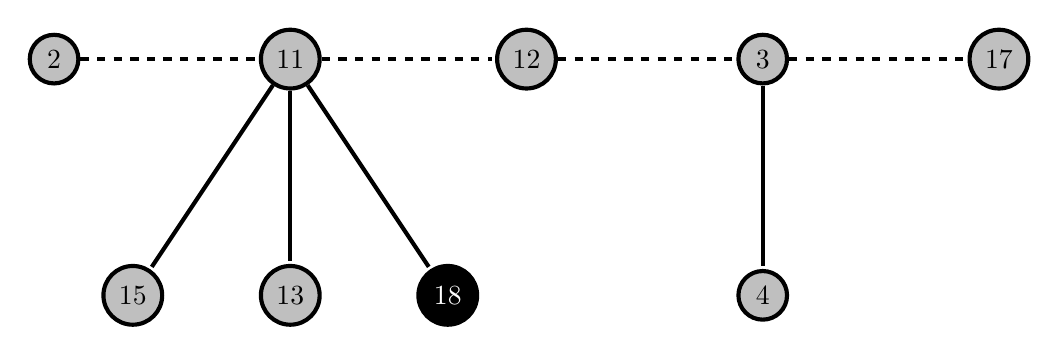
\begin{tikzpicture}[-,>=stealth,shorten >=1pt,auto,
      main node/.style={circle,draw}, line width=1.5pt]
  \node[main node,fill=lightgray] (a) at (0,0) {2};
  \node[main node,fill=lightgray] (b) at (3,0) {11};
  \node[main node,fill=lightgray] (f) at (1,-3) {15};
  \node[main node,fill=lightgray] (g) at (3,-3) {13};
  \node[main node,fill=black,text=white] (h) at (5,-3) {18};
  \node[main node,fill=lightgray] (c) at (6,0) {12};
  \node[main node,fill=lightgray] (d) at (9,0) {3};
  \node[main node,fill=lightgray] (i) at (9,-3) {4};
  \node[main node,fill=lightgray] (e) at (12,0) {17};
  \path[every node/.style={font=\small}]
  (a) edge[dashed] (b)
  (b) edge[dashed] (c)
  (c) edge[dashed] (d)
  (d) edge[dashed] (e)
  (b) edge (f)
  (b) edge (g)
  (b) edge (h)
  (d) edge (i)
  ;
  \end{tikzpicture}
  \end{center}

Which of the operations on $H$ below cause the value of the potential function to \emph{increase}?
(Note that CLRS does not contain pseudocode for {\sc Fib-Heap-Minimum}, only a written description.)
\multipleanswers
\optionsstart
\answer {\sc Fib-Heap-Minimum}($H$)
\answer {\sc Fib-Heap-Insert}($H$, 1) \correct
\answer {\sc Fib-Heap-Insert}($H$, 20) \correct
\answer {\sc Fib-Heap-Delete}($H$, 4)
\answer {\sc Fib-Heap-Delete}($H$, 18)
\answer {\sc Fib-Heap-Decrease-Key}($H$, 11, 7)
\optionsend

\explanation{
{\sc Fib-Heap-Minimum}(H) does not change the data structure and therefore does not change the potential function either.
The {\sc Fib-Heap-Insert} operations increase the length $t(H)$ of the root list by 1, and hence also $\Phi(H)$.
  {\sc Fib-Heap-Delete} operations \emph{can} result in new marked nodes, but in this case no nodes are marked because only nodes in the root list lose a child.
  The {\sc Fib-Heap-Decrease-Key} operation does not result in any {\sc Cut} operation, so the potential function does not change.

}



\question{Rod cutting}
Consider the algorithm {\sc Bottom-Up-Cut-Rod} described in CLRS Section 14.1.
Which array~$r$ does the algorithm return on input $p = \langle 2, 3, 5, 7, 11, 12 \rangle$, with $n=6$?
\oneanswer
\optionsstart
\answer $r = \langle0,2,4,6,8,10,12\rangle$
\answer $r = \langle0,2,4,6,8,11,12\rangle$
\answer $r = \langle0,2,4,6,8,11,13\rangle$ \correct
\answer $r = \langle0,2,4,6,9,12,13\rangle$
\answer $r = \langle0,2,4,6,9,12,14\rangle$
\answer $r = \langle0,2,4,6,9,13,14\rangle$
\optionsend

\explanation{
Before the first iteration we have $r[0] = 0$.
After 1 iteration we have $r[1] = 2$ (the maximum is obtained by taking 1 piece of length 1).
After 2 iterations we have $r[2] = 4$ (the maximum is obtained by taking 2 pieces of length 1).
After 3 iterations we have $r[3] = 6$ (the maximum is obtained by taking 3 pieces of length 1).
After 4 iterations we have $r[4] = 8$ (the maximum is obtained by taking 4 pieces of length 1).
After 5 iterations we have $r[5] = 11$ (the maximum is obtained by taking a piece of length 5; other solutions give a value of at most~10).
After 6 iterations we have $r[6] = 13$ (the maximum is obtained by taking a piece of length 5 and one of length 1; other solutions give a value of at most 12).
}


\question{Huffman codes}
We consider the algorithm for constructing Huffman codes in CLRS Section 15.3, run on the alphabet $C =\{a, b, c, d, e\}$ with frequencies $f_a=50$, $f_b=42$, $f_c=11$, $f_d=22$, $f_e=33$.
How long is the \emph{shortest} codeword in the computed Huffman code?
\oneanswer
\optionsstart
\answer Length 1
\answer Length 2 \correct
\answer Length 3
\answer Length 4
\optionsend

\explanation{The algorithm computes this tree (drawn without 0-1 labels on the edges), which contains three codewords (for a, b, e) of length 2 but no codewords of length 1:\medskip
\begin{center}
    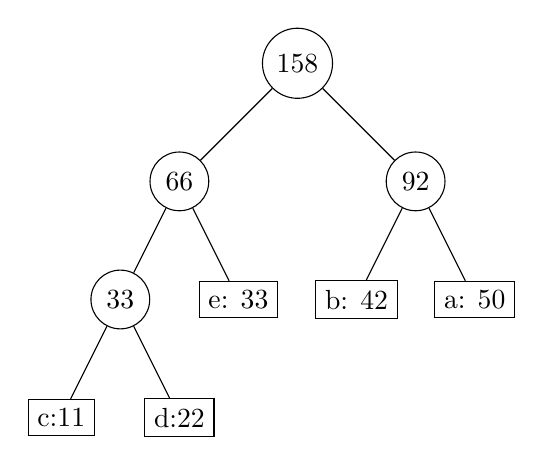
\begin{tikzpicture}[level distance=1.5cm,  level 1/.style={sibling distance=3cm},  level 2/.style={sibling distance=1.5cm}]
        \node [circle, draw] {158}
          child {node [circle, draw] {66}
            child {node [circle, draw] {33}
              child {node [rectangle, draw] {c:11}}
              child {node [rectangle, draw] {d:22}}
            }
            child {node [rectangle, draw] {e: 33}}
          }
          child {node [circle, draw] {92}
            child {node [rectangle, draw] {b: 42}}
            child {node [rectangle, draw] {a: 50}}
          };
      \end{tikzpicture}
\end{center}


}



\question{Red-black search trees I}
Consider a red-black binary search tree $T$, as described in CLRS Chapter 13.
Consider the tree below, in which all leaves are omitted (as in CLRS Figure 13.1.c) and one internal node is unspecified:

\begin{center}
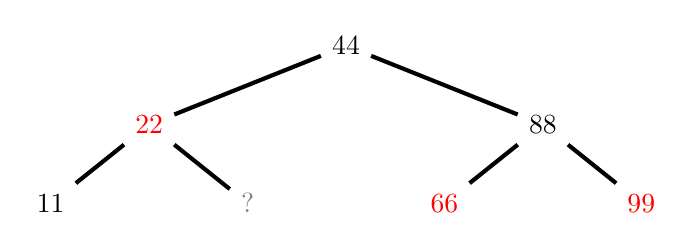
\begin{tikzpicture}[-,>=stealth,level/.style={sibling distance = 5cm/#1,
    level distance = 1cm}, line width=1.5pt]
  \node [black] {44}
      child{ node [red] {22}
              child{ node [black] {11}
              }
              child{ node [gray] {?}
              }
      }
      child{ node [black] {88}
            child{ node [red] {66}}
            child{ node [red] {99}}
          }
  ;
  \end{tikzpicture}
\end{center}

\medskip

Which nodes are possible at the position marked with ?, if the tree must satisfy the invariants of a red-black binary search tree?
\oneanswer
\optionsstart
\answer Black nodes with value at least 11 and at most 22
\answer Black nodes with value at least 22 and at most 44 \correct
\answer Black nodes with value at least 11 and at most 66
\answer Red nodes with value at least 11 and at most 22
\answer Red nodes with value at least 22 and at most 44
\answer Red nodes with value at least 11 and at most 66
\optionsend
\explanation{ The node must be black because its parent is red; otherwise a red-black invariant would be violated.
The value must be between 22 and 44 because the tree is a search tree.
}




\question{Red-black search trees II}
Consider a red-black binary search tree $T$, as described in CLRS Chapter 13.
Which statements hold for every red-black binary search tree?
\multipleanswers
\optionsstart
\answer The height and the black-height are always the same for a leaf (an external node). \correct
\answer The black-height increases by 1 when going one step up in the tree.
\answer The number of red nodes is always smaller than the number of black nodes (including leaves).  \correct
\answer The root is always black. \correct
\answer There can be both red and black leaves (external nodes).
\answer When a node is inserted it is red, and it stays red until a later insertion or deletion.
\answer When a node is deleted, it is always necessary to recolor and/or rotate.
\optionsend

\explanation{
  1. External nodes have no children and their height is therefore 0. The black-height of a node X is the number of black nodes on any simple path from, but not including, X down to a leaf; by the red-black properties this number is the same for all such paths. If X is an external node, its black-height therefore equals 0.
  2. The black-height of a red node equals the black-height of its parent.
  3. Both children of a red node are always black, and since every node has at most one parent, there are at least twice as many black nodes as red nodes. Since there is always at least one black node (e.g., the root or a leaf), the number of red nodes is always less than the number of black nodes.
  4. By the definition of a red-black BST.
  5. By the definition of red-black trees, external nodes are always black.
  6. Simple counterexample: When a node is inserted into an empty red-black tree, it is colored red. Its color is changed to black because it is the root.
  7. Simple counterexample: If the node being deleted is red and both its children are leaves (e.g., a red node whose parent is a black root), it is simply removed, without any recoloring or rotation, because none of the red-black properties is violated. In CLRS's {\sc RB-Delete}, {\sc RB-Delete-Fixup} is called only when the node removed or moved is black.
}



\question{Minimum spanning tree}
Consider the minimum spanning tree problem on this graph:
\begin{center}
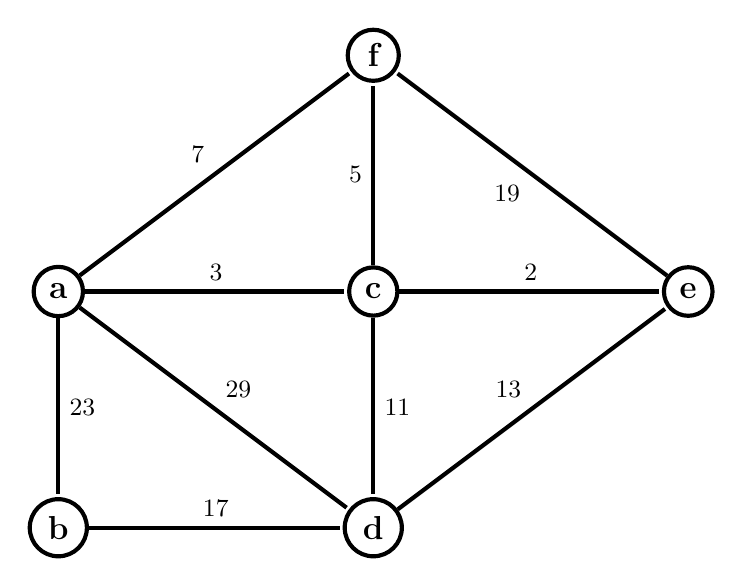
\begin{tikzpicture}[-,>=stealth,shorten >=1pt,auto,
  main node/.style={circle,draw,font=\large\bfseries}, line width=1.5pt]
\node[main node] (a) at (2,1.5) {a};
\node[main node] (b) at (2,-1.5) {b};
\node[main node] (c) at (6,1.5) {c};
\node[main node] (d) at (6,-1.5) {d};
\node[main node] (e) at (10,1.5) {e};
\node[main node] (f) at (6,4.5) {f};

\path[every node/.style={font=\small}]
(a) edge node {23} (b)
edge node {3} (c)
edge node {29} (d)
edge node {7} (f)
(b) edge node {17} (d)
(c) edge node {11} (d)
edge node {2} (e)
edge node {5} (f)
(d) edge node {13} (e)
(e) edge node {19} (f);
\end{tikzpicture}
\end{center}
Which edges belong to the minimum spanning tree (which is unique)?
\multipleanswers
\optionsstart
\answer \{a,b\}
\answer \{a,c\} \correct
\answer \{a,d\}
\answer \{a,f\}
\answer \{b,d\} \correct
\answer \{c,d\} \correct
\answer \{c,e\} \correct
\answer \{c,f\} \correct
\answer \{d,e\}
\answer \{e,f\}
\optionsend
\explanation{The minimum spanning tree can be found by running, e.g., Kruskal's or Prim's algorithm. Kruskal's algorithm adds the edges in order of weight, i.e., it starts with \{c,e\}, \{a,c\}, \{c,f\}, skips \{a,f\} because it would create a cycle, adds \{c,d\}, skips \{d,e\} because it would create a cycle, and finishes with \{b,d\}. }



\question{Cuts and safe edges}
Consider the following undirected, weighted graph with vertex set $V=\{a,b,c,d,e,f\}$:\\
\begin{center}
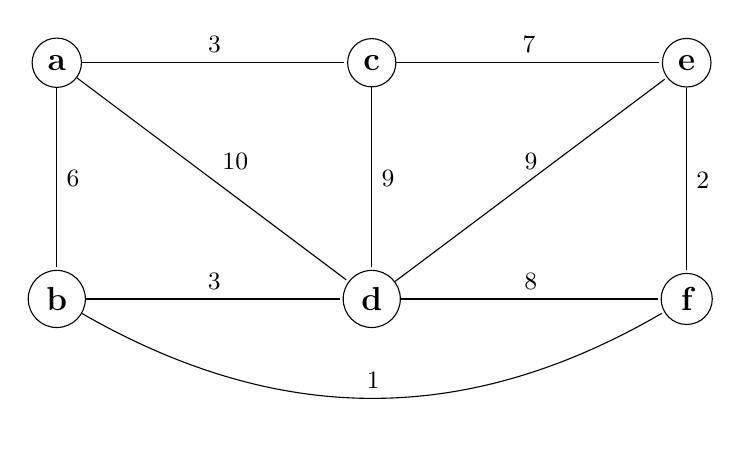
\begin{tikzpicture}[-,>=stealth,shorten >=1pt,auto,
    main node/.style={circle,draw,font=\large\bfseries}]
\node[main node] (a) at (2,1.5) {a};
\node[main node] (b) at (2,-1.5) {b};
\node[main node] (c) at (6,1.5) {c};
\node[main node] (d) at (6,-1.5) {d};
\node[main node] (e) at (10,1.5) {e};
\node[main node] (f) at (10,-1.5) {f};

\path[every node/.style={font=\small}]
(a) edge node {6} (b)
edge node {3} (c)
edge node {10} (d)
(b) edge node {3} (d)
edge[bend right=30] node {1} (f)
(c) edge node {9} (d)
edge node {7} (e)
(d) edge node {8} (f)
(e) edge node {2} (f)
(d) edge node[above] {9} (e);
\end{tikzpicture}
\end{center}
%
Which edges are light edges for the cut $(S,V-S)$, where $S=\{a,b,e,f\}$?
\multipleanswers
\optionsstart
\answer \{a,b\}
\answer \{a,c\} \correct
\answer \{a,d\}
\answer \{b,d\} \correct
\answer \{b,f\}
\answer \{c,d\}
\answer \{c,e\}
\answer \{d,e\}
\answer \{d,f\}
\answer \{e,f\}
\optionsend
\explanation{The minimum weight of edges crossing the cut is 3, and the two crossing edges \{a,c\} and \{b,d\} have this weight.
The edges \{b,f\} and \{e,f\} have lower weights but do not cross the cut.
}



\question{Choice of algorithm}
Consider the following directed, weighted graph:
\begin{center}
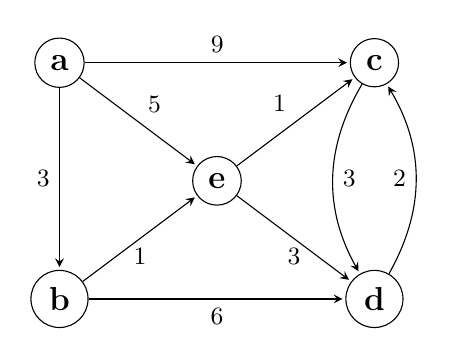
\begin{tikzpicture}[->,>=stealth,shorten >=1pt,auto,
    main node/.style={circle,draw,font=\large\bfseries}]
\node[main node] (a) at (2,1.5) {a};
\node[main node] (b) at (2,-1.5) {b};
\node[main node] (c) at (6,1.5) {c};
\node[main node] (d) at (6,-1.5) {d};
\node[main node] (e) at (4,0) {e};
\path[every node/.style={font=\small}]
(a) edge node[left] {3} (b)
edge node[above] {9} (c)
edge node {5} (e)
(b) edge node[below] {6} (d)
edge node[below] {1} (e)
(c) edge[bend right] node {3} (d)
(d) edge[bend right] node {2} (c)
(e) edge node {1} (c)
edge node[below] {3} (d);
\end{tikzpicture}
\end{center}

\medskip\noindent
Which of the algorithms from CLRS below is the best choice for computing a shortest path (single-source shortest path) from source vertex {\bf a} to destination vertex {\bf d}? Emphasis is on correctness and good asymptotic running time of the chosen algorithm. You may assume that the edge weights, as in the graph above, are between 1 and 9.
\oneanswer
\optionsstart
\answer The Bellman-Ford algorithm
\answer Breadth-first search
\answer Dijkstra's algorithm \correct
\answer Kruskal's algorithm
\answer Prim's algorithm
\optionsend
\explanation{The Bellman-Ford algorithm and Dijkstra's algorithm both compute a shortest path, but since the graph has no negative weights, Dijkstra is a better choice because it is asymptotically faster.}



\question{Shortest paths}
Consider the single-source shortest-paths problem with source vertex {\bf a} on the following graph:
\begin{center}
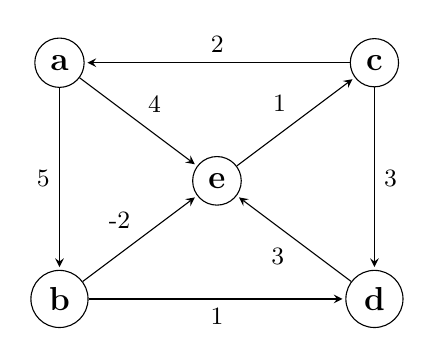
\begin{tikzpicture}[->,>=stealth,shorten >=1pt,auto,
    main node/.style={circle,draw,font=\large\bfseries}]
\node[main node] (a) at (2,1.5) {a};
\node[main node] (b) at (2,-1.5) {b};
\node[main node] (c) at (6,1.5) {c};
\node[main node] (d) at (6,-1.5) {d};
\node[main node] (e) at (4,0) {e};
\path[every node/.style={font=\small}]
(a) edge node[left] {5} (b)
edge node {4} (e)
(b) edge node[below] {1} (d)
edge node {-2} (e)
(c) edge node {3} (d)
edge node[above] {2} (a)
(d) edge node {3} (e)
(e) edge node {1} (c);
\end{tikzpicture}
\end{center}

\medskip\noindent
Which edges belong to the shortest-path tree with source vertex {\bf a}?
\multipleanswers
\optionsstart
\answer (a,b) \correct
\answer (a,e)
\answer (b,d) \correct
\answer (b,e) \correct
\answer (c,a)
\answer (c,d)
\answer (d,e)
\answer (e,c) \correct
\optionsend
\explanation{Since there are negative weights, the edges of the tree can be found by running the Bellman-Ford algorithm, which gives the stated output (which in this case is unique).}




\question{Computational geometry}
The convex hull of a set of points can be computed with algorithms from CLRS online Chapter 33.
Consider the point set $P$ below:
\begin{center}
\begin{tikzpicture}[scale=0.5]

% Manually define coordinates for points
\coordinate (p1) at (2, 3);
\coordinate (p2) at (5, 7);
\coordinate (p3) at (8, 1);
\coordinate (p4) at (1, 6);
\coordinate (p5) at (4, 5);
\coordinate (p6) at (7, 2);
\coordinate (p7) at (3, 8);
\coordinate (p8) at (6, 4);
\coordinate (p9) at (9, 9);

% Draw and label points
\foreach \i in {1,2,...,9} {
    \fill (p\i) circle (2pt) node[above] {$p_\i$};
}
\end{tikzpicture}
\end{center}

\noindent
Which statements are correct? (The first two concern the point set $P$; the others concern general point sets.)
\multipleanswers
\optionsstart
\answer The convex hull of $P$ has $h=5$ vertices. \correct
\answer The point $p_2$ is not a vertex of the convex hull of $P$. \correct
\answer Graham's scan is never asymptotically slower than Jarvis's march.
\answer Jarvis's march takes time $\Theta(n^2)$ on a worst-case input with $n$ points. \correct
\answer Graham's scan takes time $\Theta(n^2)$ on a worst-case input with $n$ points.
\optionsend
\explanation{The convex hull has the vertices $p_4,p_7,p_9,p_3,p_1$; the other points are inside the convex hull. Graham's scan is slower than Jarvis's march when the number of vertices of the convex hull is $h=o(\log n)$. When $h=\Theta(n)$, e.g., if all points lie on a circle, Jarvis's march takes $\Theta(n^2)$ time. Graham's scan takes $O(n \log n)$ time.}


\multiplechoiceend

\newpage


\section*{Written problems}\label{sec:written}

% Machine translated from the Danish original, ../danish/skriftlige.tex
{\bf Written problems:} \placeholder{How the answers are submitted, e.g.\ the file format and exam system, and whether drawings made on a tablet may be inserted.}
\begin{itemize}
    \item Use \emph{one page for each subquestion, in the same order as in the problem set.}
    \item The number/letter of the subquestion (e.g.\ 19 or 20.a) must be stated.
\end{itemize}



\section{Longest common subsequence (5\%)}

We consider the algorithm for longest common subsequence in CLRS Section 14.4.

\subquestion{a)}{
Draw the array $c$ that the algorithm fills in on the following input:
\begin{center}
$X = \langle N, E, O, N\rangle $ and $Y = \langle A, N, N, O, N, A\rangle$.
\end{center}
\medskip
\noindent
Add arrows ($\uparrow$, $\nwarrow$, $\leftarrow$) that explain the numbers in $c$, as in CLRS Figure 14.8, and \emph{state the longest common subsequence}.
}

\explanation{For clarity, we include the two strings along the edge of $c$, as in CLRS Figure 14.8.\medskip
\begin{center}
\begin{tabular}{c||c|c|c|c|c|c|c||}
    & & A & N & N & O & N & A \\
    \hline
    \hline
     & 0 & 0 & 0 & 0 & 0 & 0 & 0\\
     \hline
    N & 0 & $\uparrow$0 & $\nwarrow$1 & $\nwarrow$1 & $\leftarrow$1 & $\nwarrow$1 & $\leftarrow$1\\
    \hline
    E & 0 & $\uparrow$0 & $\uparrow$1 & $\uparrow$1 & $\uparrow$1 & $\uparrow$1 & $\uparrow$1\\
    \hline
    O & 0 & $\uparrow$0 & $\uparrow$1 & $\uparrow$1 & $\nwarrow$2 & $\leftarrow$2 & $\leftarrow$2\\
    \hline
    N & 0 & $\uparrow$0 & $\nwarrow$1 & $\nwarrow$2 & $\uparrow$2 & $\nwarrow$3 & $\leftarrow$3\\
    \hline
    \hline
\end{tabular}
\end{center}
(In some cases there is a choice between $\uparrow$ and $\leftarrow$; this does not matter when points are awarded.) The longest common subsequence is NON.
}




\section{Proof by induction of a running time (8\%)}

An algorithm takes time $T(n) = n^2 + \sum_{i=1}^n \binom{i+1}{2}$ on an input of size $n$, where $\binom{i+1}{2} = \tfrac{i(i+1)}{2}$.
We want to show that the running time satisfies $T(n) \leq 2\, n^3$ for all $n\geq 1$.

\subquestion{a)}{ Show that $T(1) = 2$.
}
\explanation{$T(1) = 1^2 + \sum_{i=1}^1 \binom{i+1}{2} = 2$.}

\subquestion{b)}{ Show $T(n) \leq 2 n^3$ by induction.
}
\explanation{
From part a) we know that $T(n) \leq 2\, n^3$ holds in the base case $n=1$.
In the inductive step we assume that $T(n-1) \leq 2\, (n-1)^3$ (inductive hypothesis).
We have
\begin{align*}
T(n) & = n^2 + \sum_{i=1}^n \tbinom{i+1}{2}\\
& = T(n-1) + (2n-1) + \tbinom{n+1}{2}\\
& \leq 2 (n-1)^3 + (2n - 1) + \tfrac{n(n+1)}{2}\\
& = (2\, n^3 - 6n^2 + 6n - 2) + (2n - 1) + (n^2 / 2 + n/2)\\
& = 2\, n^3 - 5.5 n^2 + 8.5n - 2.5\\
& < 2\, n^3 \enspace .
\end{align*}
The first inequality uses the inductive hypothesis; the second uses that $- 5.5 n^2 + 8.5n - 2.5$ is negative for $n\geq 2$.
This completes the inductive step.
}



\section{Running time (9\%)}

Assume in the following that $A[1: n]$ is an array of $n$ integers and that $k$ is an integer.
We consider these two functions:
\begin{codebox}
    \Procname{$\proc{PrefixSum}(A, n, k)$}
    \li $s = 0$
    \li \If $k > n$ \Do
    \li $t = n$ \End
    \li \Else \Do
    \li $t=k$ \End
    \li \For $i = 1$ \To $t$ \Do
    \li $s = s + A[i]$ \End
    \li \Return $s$
\end{codebox}
\begin{codebox}
  \Procname{$\proc{PowerSums}(A, n)$}
  \li $k = 1$
  \li $s = 0$
  \li \While $k < n$ \Do
  \li $s = s + \proc{PrefixSum}(A, n, k)$
  \li $k = 2\cdot k$ \End
  \li \Return $s$
\end{codebox}


\subquestion{a)}{ Give an asymptotic bound on the running time of {\sc PrefixSum} using big-$\Theta$ notation, as a function of the variables $n$ and $k$. Briefly justify your answer.}

\explanation{
The running time is $\Theta(\min(n,k))$ because the {\bf for} loop makes $t$ iterations, each iteration takes constant time, and the {\bf if} statement in lines 2-5 ensures that $t=\min(n,k)$.}

\subquestion{b)}{ Give the number of iterations of the {\bf while} loop in {\sc PowerSums} using big-$\Theta$ notation, as a function of $n$. Briefly justify your answer.}

\explanation{
The loop starts with $k=1$, doubles the value of $k$ in each iteration, and terminates when $k \geq n$.
By the definition of the binary logarithm of $n\geq 1$, the number of iterations is exactly $\lceil \lg n\rceil$.
That is, the number of iterations is $\Theta(\lg n)$.
}

\subquestion{c)}{ Give an upper bound on the running time of {\sc PowerSums} and express it in big-$\Theta$ notation, as a simple function of $n$. Briefly justify your answer.}

\explanation{
By question a), and because $k<n$, the cost of each call is $\Theta(k)$.
In iteration $i=0,1,\dots,\lceil \lg n\rceil-1$ we have $k=2^i$, so using part b) the total cost becomes  $\Theta(\sum_{i=0}^{\lceil \lg n\rceil-1} 2^i)$, which is $\Theta(n)$ since the sum is a geometric series dominated by its largest term $2^{\lceil \lg n\rceil-1} < n$.
This analysis is tight since the last call of {\sc PrefixSum} has $k \geq n/2$, and this call alone takes time $\Omega(n)$.
}






\section{Minimax spanning tree (6\%)}\label{sec:last}
Consider a weighted, undirected, connected graph $G=(V,E)$. A spanning tree of $G$ in which the weight of the heaviest edge is as small as possible is called a \emph{MiniMax Spanning Tree} (MMST).

\medskip
\noindent
{\bf Example:} In this graph the highlighted edges form an MMST. The maximum weight in the tree is 4, and there is no spanning tree with a smaller maximum weight.

\begin{center}
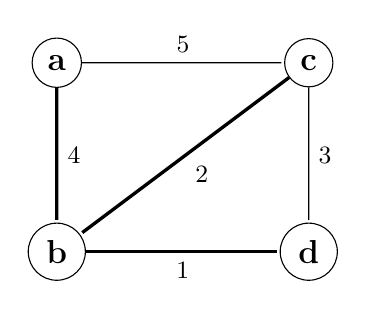
\begin{tikzpicture}[-,scale=0.8,>=stealth,shorten >=1pt,auto,
  main node/.style={circle,draw,font=\large\bfseries}]
\node[main node] (a) at (2,1.5) {a};
\node[main node] (b) at (2,-1.5) {b};
\node[main node] (c) at (6,1.5) {c};
\node[main node] (d) at (6,-1.5) {d};

\path[every node/.style={font=\small}]
(a) edge[very thick] node {4} (b)
edge node {5} (c)
(b) edge[very thick] node[below] {1} (d)
(c) edge node {3} (d)
edge[very thick] node {2} (b);
\end{tikzpicture}
\end{center}


\subquestion{a)}{ Give an example showing that an MMST is not always a minimum spanning tree.}

\explanation{ In this graph there is an MMST with maximum weight 2 and total weight 4. A minimum spanning tree has weight 3.
  \begin{center}
    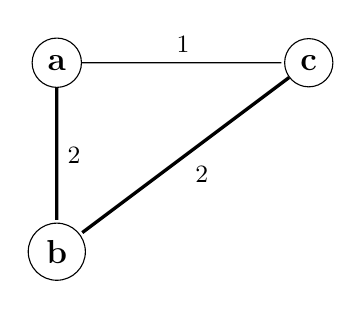
\begin{tikzpicture}[scale=0.8,-,>=stealth,shorten >=1pt,auto,
      main node/.style={circle,draw,font=\large\bfseries}]
    \node[main node] (a) at (2,1.5) {a};
    \node[main node] (b) at (2,-1.5) {b};
    \node[main node] (c) at (6,1.5) {c};

    \path[every node/.style={font=\small}]
    (a) edge[very thick] node {2} (b)
    edge node {1} (c)
    (c) edge[very thick] node {2} (b);
    \end{tikzpicture}
    \end{center}
}

\subquestion{b)}{ Prove that a minimum spanning tree is always an MMST. }

\explanation{Proof by contradiction.
Let $T$ denote a minimum spanning tree (MST) and assume that it is not an MMST.
Let $T'$ denote an MMST.
Let $e$ denote the edge of largest weight in $T$ and let $e'$ denote the edge of largest weight in $T'$. Since $T$ is not an MMST, we must have $|e| > |e'|$, and $e$ is not in $T'$.
When $e$ is added to $T'$, a cycle is formed.
This cycle contains an edge that crosses the cut defined by the connected components that arise if $e$ is removed from $T$, i.e., $e$ is not minimal in the cut, contradicting the assumption.
%All edges in this cycle have smaller weight than $e$.
%This means that every cut with $e$ as a crossing edge contains an edge of smaller weight than the weight of $e$.
%In other words, $e$ is not a safe edge for any cut.
%But then $e$ cannot be in any MST.
%This contradicts the fact that $e$ is in $T$.
}


\label{page:last}
